\documentclass[xcolor=dvipsnames]{beamer}

%\setbeamercovered{transparent}
\setbeamertemplate{footline}{}
\defbeamertemplate*{headline}{miniframes theme no subsection} %Esto remueve la barra de subsection
{%
  \begin{beamercolorbox}[colsep=1.5pt]{upper separation line head}
  \end{beamercolorbox}
  \begin{beamercolorbox}{section in head/foot}
    \vskip2pt\insertnavigation{\paperwidth}\vskip2pt
  \end{beamercolorbox}%
  \begin{beamercolorbox}[colsep=1.5pt]{lower separation line head}
  \end{beamercolorbox}
}

\usepackage{amsmath} %necesario para equation*
\usepackage{amsthm} %necesario para proof enviroment
\usepackage{lipsum} %para usar el texto de relleno
\usepackage{amsfonts} %para Z estilizada
\usepackage{mdframed}
\usepackage{xcolor}
\usepackage{tikz}
\usepackage{mdframed} %para los cuadrados de los teoremas
\usepackage{tikz-cd} %para los diagramas conmutativos
\usepackage{multicol} %varias columnas
\usepackage{adjustbox}

\usefonttheme{professionalfonts} % using non standard fonts for beamer
\usefonttheme{serif} % default family is serif

\definecolor{LightGrayHeader}{RGB}{220, 220, 220}
\definecolor{LightGrayBG}{RGB}{250, 250, 250}
\definecolor{FancyBlue}{RGB}{28, 93, 105}
\setbeamercolor{frametitle}{fg=Black} %Título frame, fondo títuo frame
\setbeamercolor{background canvas}{bg=LightGrayBG}
\setbeamercolor{section in head/foot}{fg=Black, bg=LightGrayHeader}
\setbeamercolor{lower separation line head}{bg=FancyBlue}
\setbeamercolor{block title}{fg=FancyBlue}
\setbeamercolor{item}{fg=FancyBlue}
\setbeamercolor{qed symbol}{fg=FancyBlue}
\setbeamercolor{title}{fg=FancyBlue}
\setbeamercolor{alerted text}{fg=FancyBlue}
%\setbeamercolor{block title}{bg=White}
%\setbeamercolor{block body}{bg=White}

\setbeamerfont{frametitle}{series=\scshape}

%\newtheorem{teorema}{Teorema}

\newmdtheoremenv{Tma}{Teorema}
\newmdtheoremenv{prop}{Proposición}
\newmdtheoremenv{Lema}{Lema}
\newmdtheoremenv{Hecho}{Hecho}
\newmdtheoremenv{Def}{Definición}
\newtheorem{obs}{Observación}
\renewcommand*{\proofname}{Prueba}

\makeatletter
\newenvironment<>{myproof}[1][\proofname]{%
  \par
  \def\insertproofname{#1\@addpunct{.}}%
  \pushQED{\qed}
  \large{\textcolor{FancyBlue}{\insertproofname}} \vspace{0.15cm} \hspace*{\fill} \\}
{\popQED}
\makeatother

\title{\textsc{COMPACIDAD\\como conexión entre lógica y topología}\\ \vspace{0.5cm}
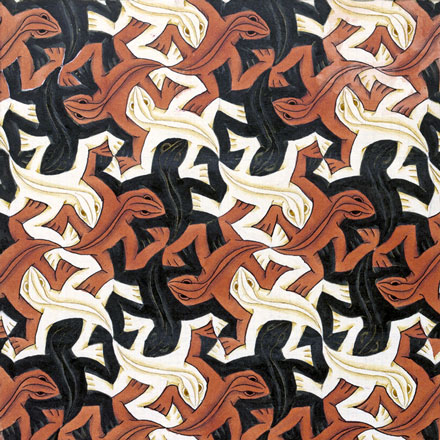
\includegraphics[width=0.4\textheight,height=0.4\textheight]{Img1.jpg} \vspace{-0.45cm}}
\author{Juan Camilo Lozano Suárez \vspace{-0.3cm}}
\institute{Universidad Nacional de Colombia \vspace{-0.3cm}}
\date{Junio 2 de 2026}

\begin{document}

\maketitle

\usebackgroundtemplate{
   \tikz[overlay,remember picture] \node[opacity=0.15, at=(current page.center)] {
   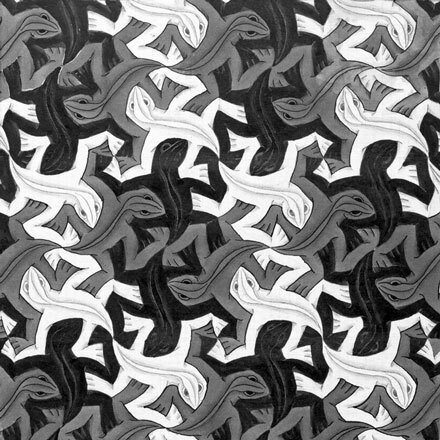
\includegraphics[height=0.6\paperheight,width=0.6\paperheight]{Img1_bw.jpg}};
}

\section{Un tema recurrente}
\begin{frame}{Un tema recurrente en matemáticas}
    \vfill
       \center{\LARGE{\alert{Local/Finito vs Global/Infinito}}}
    \vfill
\end{frame}
\begin{frame}{Compacidad}
   En topología:
   \begin{Def}
      Un espacio topológico $X$ se dice compacto si todo cubrimiento por abiertos de $X$ tiene un subcubrimiento finito.\vspace{0.3cm}
   \end{Def}
   \vspace{0.3cm}
   \onslide<2->
   En lógica:
   \begin{Tma}[De compacidad]
      Sean $L$ un lenguaje de primer orden y $\mathcal{E}$ un conjunto de $L$-sentencias.
      \center{Si $\mathcal{E}$ es finitamente satisfacible entonces $\mathcal{E}$ es satisfacible.\vspace{0.3cm}}
   \end{Tma}
\end{frame}
\begin{frame}{Compacidad}
    \begin{Tma}[De compacidad]
      Sean $L$ un lenguaje de primer orden y $\mathcal{E}$ un conjunto de $L$-sentencias.
      \center{Si $\mathcal{E}$ es finitamente satisfacible entonces $\mathcal{E}$ es satisfacible.\vspace{0.3cm}}
   \end{Tma}
   \vspace{0.3cm}
   \begin{itemize}
      \item $\mathcal{E}$ se dice finitamente satisfacible si todo subconjunto finito de $\mathcal{E}$ tiene un modelo.
      \item<2-> $\mathcal{E}$ se dice satisfacible si tiene un modelo.
   \end{itemize}
\end{frame}

\section{Demostraciones}
\begin{frame}{Demostraciones del teorema de compacidad}
   \begin{columns}
      \begin{column}{0.48\textwidth}
         % https://tikzcd.yichuanshen.de/#N4Igdg9gJgpgziAXAbVABwnAlgFyxMJZABgBpiBdUkANwEMAbAVxiRAB12cYAPHYACowIAJxgBbOgAJYUgMYRxaBjDw4mUAL4hNpdJlz5CKMgGYqtRizadufQcLGSZMeYrR05WKHS06LMFAA5vBEoABmIopIZCA4EEgAjJoUmkA
\begin{tikzcd}
\text{Teorema de completitud} \arrow[ddd] \\
                                          \\
                                          \\
\text{Teorema de compacidad}             
\end{tikzcd}

      \end{column}
      \begin{column}{0.48\textwidth}
         \begin{itemize}
            \item <2-> $\mathcal{E}$ es consistente.
            \item <3-> $\mathcal{E}$ puede ser completado: existe $\mathcal{E}^{\#}$ completo y f.s. tal que $\mathcal{E}\subseteq\mathcal{E}^{\#}$
            \item <4-> $\mathcal{E}^{\#}$ es Gödeliano. Por el teorema de completitud $\mathcal{E}^{\#}$ tiene un modelo y por tanto también $\mathcal{E}$.
         \end{itemize}
      \end{column}
   \end{columns}
\end{frame}
\begin{frame}{Demostraciones del teorema de compacidad}
   \begin{columns}
      \begin{column}{0.48\textwidth}
         \begin{tikzcd}
\text{Demostraciones topológicas} \arrow[ddd] \\
                                          \\
                                          \\
\text{Teorema de compacidad}             
\end{tikzcd}

      \end{column}
      \begin{column}{0.48\textwidth}
         \begin{itemize}
            \item Teorema de Tychonoff
            \item Conjunto de Cantor
         \end{itemize}
      \end{column}
   \end{columns}
\end{frame}
\begin{frame}{Demostraciones del teorema de compacidad}
    \begin{columns}
      \begin{column}{0.48\textwidth}
         \begin{tikzcd}
\text{Demostraciones algebraicas} \arrow[ddd] \\
                                          \\
                                          \\
\text{Teorema de compacidad}             
\end{tikzcd}

      \end{column}
      \begin{column}{0.48\textwidth}
         \begin{itemize}
            \item Álgebra de Lindembaum-Tarski
            \item Filtros
         \end{itemize}
      \end{column}
   \end{columns}
\end{frame}
\begin{frame}{Demostraciones del teorema de compacidad}
    \begin{columns}
      \begin{column}{0.48\textwidth}
         \begin{tikzcd}
\text{Demostraciones híbridas} \arrow[ddd] \\
                                          \\
                                          \\
\text{Teorema de compacidad}             
\end{tikzcd}

      \end{column}
      \begin{column}{0.48\textwidth}
         \begin{itemize}
            \item Ultraproductos y espacios de Stone
            \item Espacios de Stone de álgebras boolenas
         \end{itemize}
      \end{column}
   \end{columns}
\end{frame}

\section{Una equivalencia topológica}
\begin{frame}{Una equivalencia topológica}
   \begin{itemize}
      \item Llamamos $\mathcal{V}$ al conjunto de todas las valuaciones de $L$.
      \item <2-> Para cada sentencia $P$ se define 
         $$\mathcal{U}(P):=\left\lbrace \phi \in \mathcal{V}\mid \phi(P)=1 \right\rbrace$$
      \item <3-> El conjunto $\mathcal{B}:=\left\lbrace \mathcal{U}(P)\mid P \text{ es una sentencia}\right\rbrace$ es base para una topología sobre $\mathcal{V}$\vspace{0.3cm}
         \begin{itemize}
            \item <4-> $\mathcal{V}=\mathcal{U}(P)\cup \mathcal{U}(\neg P)$\vspace{0.3cm}
            \item <5-> $\mathcal{U}(P_1)\cap\mathcal{U}(P_2)=\mathcal{U}(P_1\wedge P_2)$
         \end{itemize}
   \end{itemize}
\end{frame}
\begin{frame}{Una equivalencia topológica}
   \begin{itemize}
      \item $\mathcal{E}$ es insatisfacible: para toda $\phi\in\mathcal{V}$ existe $P\in\mathcal{E}$ tal que $\phi(P)=0$, es decir $\phi(\neg P)=1$.
   \end{itemize}
   \onslide<2->{
      \begin{Lema}
         $\mathcal{E}$ es insatisfacible ssi $\left\lbrace \mathcal{U}(\neg P) \mid P\in \mathcal{E}\right\rbrace$ es un cubrimiento de $\mathcal{V}$\vspace{0.3cm} 
      \end{Lema}
   \vspace{0.3cm}
   }
   \only<3>{
      $(\Rightarrow)$ Supongamos que $\mathcal{E}$ es insatisfacible. Dado $\phi\in \mathcal{V}$, existe $P\in \mathcal{E}$ tal que $\phi(\neg P)=1$, luego $\phi \in \mathcal{U}(\neg P)$.
   }
   \only<4>{
      $(\Leftarrow)$ Supongamos que $\left\lbrace \mathcal{U} (\neg P) \mid P\in \mathcal{E}\right\rbrace$ es un cubrimiento de $\mathcal{V}$. Para cualquier $\phi\in \mathcal{V}$ existe $P\in\mathcal{E}$ tal que $\phi\in\mathcal{U}(\neg P)$, luego $\phi(\neg P)=1$ y $\phi(P)=0$. Entonces $\mathcal{E}$ es insatisfacible.
   }
\end{frame}
\begin{frame}{Una equivalencia topológica}
   \begin{Hecho}
       Las siguientes afirmaciones son equivalentes:
       \begin{itemize}
          \item[(1)] $L$ satisface el teorema de compacidad
          \item[(2)] El espacio de valuaciones $\mathcal{V}$ de $L$ es compacto
       \vspace{0.3cm}
       \end{itemize}
   \end{Hecho}
\end{frame}
\begin{frame}{Una equivalencia topológica}
   \begin{Hecho}
       Las siguientes afirmaciones son equivalentes:
       \begin{itemize}
          \item[(1)] Si $\mathcal{E}$ es insatisfacible entonces $\mathcal{E}$ no es finitamente satisfacible.
          \item[(2)] El espacio de valuaciones $\mathcal{V}$ de $L$ es compacto
       \vspace{0.3cm}
       \end{itemize}
   \end{Hecho}
\end{frame}
\begin{frame}{Una equivalencia topológica}
   \alert{$(1)\Rightarrow (2)$}
   \begin{itemize}
      \item Sea $\left\lbrace \mathcal{U}(P)\mid P\in \mathcal{E}\right\rbrace$ un cubrimiento abierto de $\mathcal{V}$.
      \item <2-> $\left\lbrace \mathcal{U}(P)\mid P\in \mathcal{E}\right\rbrace=\left\lbrace \mathcal{U}(\neg P)\mid P\in \mathcal{E}'\right\rbrace$ con $\mathcal{E}'=\left\lbrace \neg P \mid P\in \mathcal{E}\right\rbrace$.
      \item <3-> $\mathcal{E}'$ es insatisfacible.
      \item <4-> Existe un subconjunto finito $\mathcal{E}^{'}_{fin}\subseteq \mathcal{E}'$ que es insatisfacible.
      \item <5-> $\left\lbrace U(\neg P)\mid P\in \mathcal{E}^{'}_{fin}\right\rbrace$ es un cubrimiento abierto de $\mathcal{V}$.
      \item <6-> $\mathcal{V}$ es compacto.
   \end{itemize}
\end{frame}
\begin{frame}
   \alert{$(2)\Rightarrow (1)$}
   \begin{itemize}
      \item Supongamos que $\mathcal{E}$ es insatisfacible.
      \item <2-> $\left\lbrace U(\neg P)\mid P\in \mathcal{E}\right\rbrace$ es un cubrimiento abierto de $\mathcal{V}$.
      \item <3-> Existe un subconjunto finito $\mathcal{E}_{fin}\subseteq \mathcal{E}$ tal que $\left\lbrace U(\neg P)\mid P\in \mathcal{E}_{fin}\right\rbrace$ cubre a $\mathcal{V}$.
      \item <4-> $\mathcal{E}_{fin}$ es insatisfacible.
      \item <5-> $\mathcal{E}$ no es finitamente satisfacible.
   \end{itemize}
   \onslide<5>\hfill \qed
\end{frame}
\begin{frame}
        \frametitle{Referencias}
        \nocite{*}
        \bibliographystyle{apalike}
        \bibliography{refs}
    \end{frame}
    \begin{frame}
   \vfill
   \center{\Huge{\alert{¡MUCHAS GRACIAS!}}}
   \vfill
\end{frame}
\end{document}
